% !TEX root = ../main.tex
\section{Неперервні випадкові вектори}

\begin{definition}
    Вимірна функція $\xi(\omega): \Omega \rightarrow \mathbb{R}^n$ називається 
    \emph{неперервним випадковим вектором}, якщо координати $\xi_i$ є 
    неперервними випадковими випадковими величинами $\forall i = \overline{1,n}$.
\end{definition}
\begin{remark}
    $F_{\vec{\xi}}\left(\vec{x}\right) = 
    P\left\{\omega\;:\;\xi_1(\omega)<x_1,...,\xi_n(\omega)<x_n\right\}$ --- 
    функція розподілу, є неперервною по всім аргументам.
\end{remark}

\subsection{Щільність розподілу двовимірного неперервного випадкового вектора}
\begin{definition}
    \emph{Щільністю розподілу} двовимірного випадкового вектора називається 
    подвійна границя
    \begin{equation}
        f_{\vec{\xi}}(x, y) = \lim_{\substack{\Delta x \to 0 \\ 
        \Delta y \to 0}} \frac{P\left\{\vec{\xi} \in \Pi\right\}}
        {\Delta x \Delta y}
    \end{equation}
    де $\Pi = \left[x; x+\Delta x\right] \times \left[y; y+\Delta y\right]$.
\end{definition}
\begin{remark}
    В означенні 1 замість можна брати будь-яку обмежену замкнену область (компакт) 
    $D$ і тоді
    \begin{equation*}
        f_{\vec{\xi}}(x, y) = \lim_{S(D) \to 0} 
        \frac{P\left\{\vec{\xi} \in D\right\}}
        {S(D)}
    \end{equation*}
\end{remark}

\noindent\textbf{Зв’язок щільності розподілу з сумісною функцією розподілу: }

$f_{\vec{\xi}}(x, y) = \lim_{\substack{\Delta x \to 0 \\ 
\Delta y \to 0}} \frac{P\left\{\vec{\xi} \in \Pi\right\}}
{\Delta x \Delta y} = 
\lim_{\substack{\Delta x \to 0 \\ \Delta y \to 0}} 
\left(
    \frac{F_{\vec{\xi}}(x+\Delta x, y+\Delta y) - F_{\vec{\xi}}(x, y+\Delta y)}
    {\Delta x \Delta y}
    -
    \frac{F_{\vec{\xi}}(x+\Delta x, y) - F_{\vec{\xi}}(x, y)}
    {\Delta x \Delta y}
\right) =$

$= \left|\text{формула Лагранжа про скінченні прирости}\;|
\;\theta_1, \theta_2 \in (0, 1)\right| = $

$= \lim_{\substack{\Delta x \to 0 \\ \Delta y \to 0}} 
\left(
    \frac{\frac{\partial F}{\partial x}(x + \theta_1 \Delta x, y + \Delta y)\Delta x}
    {\Delta x \Delta y}
    -
    \frac{\frac{\partial F}{\partial x}(x + \theta_2 \Delta x, y)\Delta x}
    {\Delta x \Delta y}
\right) = 
\left|\theta_3, \theta_4 \in (0, 1)\right| =$

$= \lim_{\substack{\Delta x \to 0 \\ \Delta y \to 0}}
\frac{\frac{\partial^2 F}{\partial x \partial y}(x + \theta_3 \Delta x, 
y + \theta_4 \Delta y)\Delta y}
{\Delta y} = \frac{\partial^2 F_{\vec{\xi}}}{\partial x \partial y}(x, y)$

Таким чином, якщо $\exists \frac{\partial^2 F_{\vec{\xi}}}{\partial x \partial y}$ 
--- неперервна, то
\begin{equation}
    f_{\vec{\xi}}(x, y) = \frac{\partial^2 F_{\vec{\xi}}}{\partial x \partial y}(x, y)
\end{equation}

\begin{definition}
    Поверхня, що є графіком щільності двовимірного випадкового вектора називається 
    \emph{поверхнею розподілу}.
\end{definition}
\begin{definition}
    Лінії, де $f_\xi(x, y) = const$, називаються \emph{лініями рівних ймовірностей}.
\end{definition}

\noindent\textbf{Властивості щільності: }

\begin{enumerate}
    \item $f_{\vec{\xi}}(x, y) \geq 0$
    \item З формули 2: $F_{\vec{\xi}}(x, y) 
    = \int_{-\infty}^x \int_{-\infty}^y f_{\vec{\xi}}(r, s) 
    \,\mathrm{d}r \mathrm{d}s $
    \item Умова нормування: 
    $\int_{-\infty}^{+\infty} \int_{-\infty}^{\infty} f_{\vec{\xi}}(r, s) 
    \,\mathrm{d}r \mathrm{d}s = 1$ --- весь об'єм під поверхнею розподілу 
    дорівнює 1.
    \item $F_{\xi_1}(x) = \int_{-\infty}^{x} \int_{-\infty}^{+\infty} 
    f_{\vec{\xi}}(r, s) \,\mathrm{d}r \mathrm{d}s$

    $F_{\xi_2}(y) = \int_{-\infty}^{+\infty} \int_{-\infty}^{y} 
    f_{\vec{\xi}}(r, s) \,\mathrm{d}r \mathrm{d}s$
    \item Щільності розподілу окремих координат називаються 
    \emph{маргінальними щільностями розподілу}.

    $f_{\xi_1}(x) = F^{'}_{\xi_1}(x) 
    = \int_{-\infty}^{+\infty} f_{\vec{\xi}}(x, y) \,\mathrm{d}y $

    $f_{\xi_2}(x) = F^{'}_{\xi_2}(x) 
    = \int_{-\infty}^{+\infty} f_{\vec{\xi}}(x, y) \,\mathrm{d}x $
    
    \item D - замкнена обмежена область в $\mathbb{R}^2$.
    
    $P\left\{ \vec{\xi} \in D \right\} = \iint_D f_{\vec{\xi}}(x, y) \,
    \mathrm{d}x \mathrm{d}y$.
\end{enumerate}

\subsection{Рівномірний закон розподілу на площині}
\begin{definition}
    D --- замкнена обмежена область (компакт) в $\mathbb{R}^2$. 
    Вектор $\vec{\xi} = (\xi_1,\;\xi_2)^T$ називається 
    \emph{рівномірно розподіленим в області D}, якщо 
    \begin{equation*}
        f_{\vec{\xi}}(x, y) = 
        \begin{cases}
            \frac{1}{S(D)},&(x, y) \in D \\
            0,&(x, y) \notin D
        \end{cases}
    \end{equation*}
\end{definition}
\begin{example}
    \begin{tabular}{c m{4cm}}
        $f_{\vec{\xi}}(x, y) = 
        \begin{cases}
            2, & (x, y) \in D \\
            0, & (x, y) \notin D
        \end{cases}
        $
        &
        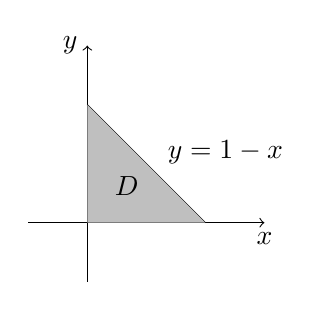
\begin{tikzpicture}[scale = 1.5]
            \draw [->] (0, -0.5) -- (0, 1.5);
            \draw [->] (-0.5, 0) -- (1.5, 0);
            \draw (1, 0) -- (0, 1);
            \fill [lightgray] (0, 0) -- (1, 0) -- (0, 1);
            \node [below] at (1.5, 0) {$x$};
            \node [left] at (0, 1.5) {$y$};
            \node [above right] at (0.15, 0.15) {$D$};
            \node [right] at (0.6, 0.6) {$y = 1 - x$};
        \end{tikzpicture}
    \end{tabular}
    
    \begin{enumerate}
        \item $f_{\xi_1}(x) = \int_{-\infty}^{+\infty} f_{\vec{\xi}}(x, y) \,\mathrm{d}y = 
        \begin{cases}
            0 , &x\leq0\\
            \int_0^{1-x} 2 \,\mathrm{d}y = 2(1-x), & 0 < x \leq 1 \\
            0, & x > 1 
        \end{cases}$

        $f_{\xi_2}(y) = \int_{-\infty}^{+\infty} f_{\vec{\xi}}(x, y) \,\mathrm{d}x = 
        \begin{cases}
            0 , &y\leq0\\
            \int_0^{1-y} 2 \,\mathrm{d}x = 2(1-y), & 0 < y \leq 1 \\
            0, & y > 1 
        \end{cases}$
        \item Функції розподілу координат: 
        
        $F_{\xi_1}(x) = \int_{-\infty}^{x} f_{\xi_1}(t) \,\mathrm{d}t $
        
        $F_{\xi_2}(y) = \int_{-\infty}^{y} f_{\xi_2}(t) \,\mathrm{d}t $
    \end{enumerate}
\end{example}